\subsubsection{Genotypes and Genotyping} \label{background:biology:genotype_and_genotyping}
The term \textit{genotype} refers to the set of variants an individual carries at a particular location along the genome sequence of all of its chromosomes \cite{nhgri_genotype}.
For humans, who have two of each chromosome, a genotype would refer to two variants, one in each of the two chromosomes.
\textit{Genotyping} an individual refers to the process of determining which genotypes an individual carries. 
In most genotyping software tools today, genotypes are given in a format that specifies whether a particular variant is present in none, one or both of a human's chromosomes.
For instance, given a reference genome sequence where a variant site is known to could manifest an A at a particular allele where the reference sequence contains a C, a human individual's genotype for this variant could either be referred to as $0/0$, meaning that the variant is present in neither of the chromosomes, $0/1$, meaning that the variant is present in one of the chromosomes, or $1/1$, meaning that the variant is present in both chromosomes.

\definecolor{variantcolor}{RGB}{235,235,235}

\begin{figure}[H]
\begin{center}
\scalebox{0.85}{
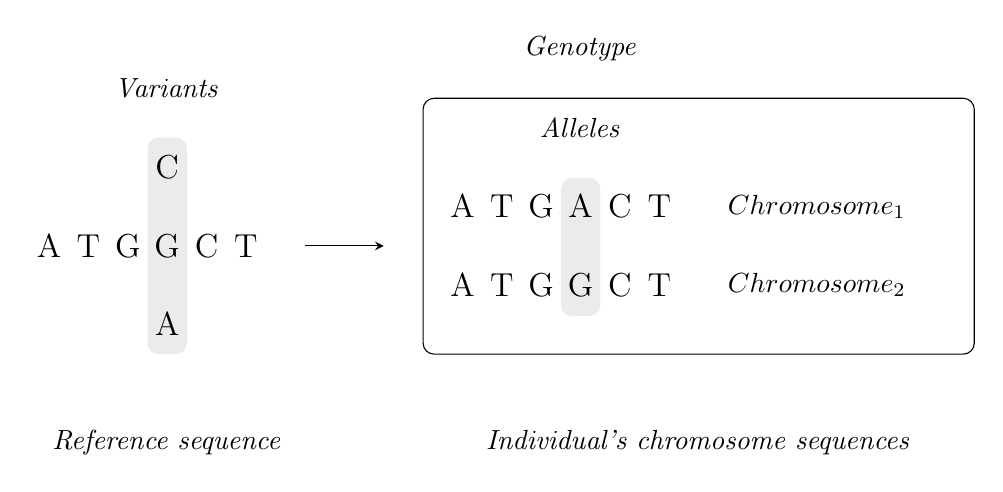
\begin{tikzpicture}
  % Variants
  \node at(2.25,2)(title){\textit{Variants}};
  \node at(2.25,0)[rounded corners,minimum width=0.5cm,minimum height=2.75cm, fill=variantcolor](variant){};
  % Sequence (left)
  \node at(0.75,0)(n2){\large A};
  \node at(1.25,0)(n3){\large T};
  \node at(1.75,0)(n4){\large G};
  \node at(2.25,1)(n5){\large C};
  \node at(2.25,0)(n5){\large G};
  \node at(2.25,-1)(n5){\large A};
  \node at(2.75,0)(n5){\large C};
  \node at(3.25,0)(n5){\large T};
  % Arrow
  \draw [-stealth](4,0) -- (5,0);
  % Genotype
  \node at(7.5,2.5)(title){\textit{Genotype}};
  \node at(9,0.25)[rectangle,rounded corners,draw,minimum width=7cm,minimum height=3.25cm](genotype){};
  % Alleles 
  \node at(7.5,1.5)(title){\textit{Alleles}};
  % Chromosomes
  \node at(10.5,0.5)(title){$Chromosome_1$};
  \node at(10.5,-0.5)(title){$Chromosome_2$};
  \node at(7.5,-.015)[rounded corners,minimum width=0.5cm,minimum height=1.75cm, fill=variantcolor](variant){};
  % Chromosome 1 sequence
  \node at(6,0.5)(n2){\large A};
  \node at(6.5,0.5)(n3){\large T};
  \node at(7,0.5)(n4){\large G};
  \node at(7.5,0.5)(n5){\large A};
  \node at(8,0.5)(n5){\large C};
  \node at(8.5,0.5)(n5){\large T};
  % Chromosome 2 sequence
  \node at(6,-0.5)(n2){\large A};
  \node at(6.5,-0.5)(n3){\large T};
  \node at(7,-0.5)(n4){\large G};
  \node at(7.5,-0.5)(n5){\large G};
  \node at(8,-0.5)(n5){\large C};
  \node at(8.5,-0.5)(n5){\large T};
  % Reference and the individual's chromosomes
  \node at(2.25,-2.5)(ref){\textit{Reference sequence}};
  \node at(9,-2.5)(ind){\textit{Individual's chromosome sequences}};
\end{tikzpicture}
}
\caption{In humans, where there are two chromosomes, a genotype constitutes as a set of two alleles, one in each chromosome at the variant location. Along the reference sequence on the left, several possible variants may be known to occur at a specific location. After examining the sequence of an individual, we try to determine the individual's genotype by scoring which variants are present in each chromosome at the location of interest.}
\label{figure:variant_and_genotype}
\end{center}
\end{figure}

The most established way to genotype an individual today is to align DNA reads to a reference genome sequence and then examine how the reads differ from the reference sequence to determine which variants are present, and which genotypes are most probable at the different locations \cite{gatk}.
However, given how many reads one have come to expect from high-throughput sequencing today [\ref{background:biology:high_throughput_dna_sequencing}] and how time consuming it is to align reads to a $3*10^9$ long reference sequence, although accurate, this strategy is very compute- and time consuming.
A new prominent strategy has emerged in recent years that helps to alleviate the compute- and time consumption aspect of genotyping.
Statistics based methods, usually referred to \textit{alignment-free} genotyping methods, where the variant calling step where reads are aligned to the reference genome is skipped altogether. 
In such methods, small parts of the sequenced reads called \textit{k}mers are analyzed, and bayesian models are then used to determine which genotypes are most probable given the results from the \textit{k}mer analysis and previous knowledge accumulated over years of research \cite{kage,malva,1000_genomes_project}.
One such bayesian genotyper, KAGE, have recently showed that it can genotype a human individual more than 10 times faster than any other known genotyper tool, while still providing competitive accuracy scores \cite{kage}.
